\documentclass[letterpaper,12pt,fleqn]{article}
\usepackage{matharticle}
\usepackage{graphtheory}
\pagestyle{empty}
\begin{document}
\section*{1.2: Connected Graphs}

\begin{enumerate}[start=11]
\item Let \(G\) be the graph in Figure 1.20, let \(X=\set{e,f}\), where \(e=ru\) and \(f=vw\), and let \(U=\set{u,w}\).
  Draw the subgraphs \(G-X\) and \(G-U\) of \(G\).

  \bigskip

  \begin{center}
    \begin{tikzpicture}
      \begin{scope}[every node/.style={labeled node}, node distance=1.5cm]
        \node (r) {\(r\)};
        \node (s) [right=of r] {\(s\)};
        \node (t) [right=of s] {\(t\)};
        \node (u) [below=of r] {\(u\)};
        \node (v) [right=of u] {\(v\)};
        \node (w) [right=of v] {\(w\)};
        \node (x) [below=of u] {\(x\)};
        \node (y) [right=of x] {\(y\)};
        \node (z) [right=of y] {\(z\)};
      \end{scope}
      \draw (r) edge node [auto] {\(e\)} (u) edge (s) edge (v);
      \draw (s) edge (t) edge (v);
      \draw (t) edge (v) edge (w);
      \draw (u) edge (v) edge (x);
      \draw (v) edge node [auto] {\(f\)} (w) edge (y);
      \draw (w) edge (z);
      \draw (x) edge (y);
      \draw (y) edge (z);
    \end{tikzpicture}

    \bigskip

    \(G\)
  \end{center}

  \begin{minipage}{3in}
    \begin{center}

      \begin{tikzpicture}
        \begin{scope}[every node/.style={labeled node}, node distance=1.5cm]
          \node (r) {\(r\)};
          \node (s) [right=of r] {\(s\)};
          \node (t) [right=of s] {\(t\)};
          \node (u) [below=of r] {\(u\)};
          \node (v) [right=of u] {\(v\)};
          \node (w) [right=of v] {\(w\)};
          \node (x) [below=of u] {\(x\)};
          \node (y) [right=of x] {\(y\)};
          \node (z) [right=of y] {\(z\)};
        \end{scope}
        \draw (r) edge (s) edge (v);
        \draw (s) edge (t) edge (v);
        \draw (t) edge (v) edge (w);
        \draw (u) edge (v) edge (x);
        \draw (v) edge (y);
        \draw (w) edge (z);
        \draw (x) edge (y);
        \draw (y) edge (z);
      \end{tikzpicture}
      
      \bigskip

      \(G-X\)
    \end{center}
  \end{minipage}
  \begin{minipage}{3in}
    \begin{center}
      \begin{tikzpicture}
        \begin{scope}[every node/.style={labeled node}, node distance=1.5cm]
          \node (r) {\(r\)};
          \node (s) [right=of r] {\(s\)};
          \node (t) [right=of s] {\(t\)};
          \node (u) [below=of r,white] {};
          \node (v) [right=of u] {\(v\)};
          \node (w) [right=of v,white] {};
          \node (x) [below=of u] {\(x\)};
          \node (y) [right=of x] {\(y\)};
          \node (z) [right=of y] {\(z\)};
        \end{scope}
        \draw (r) edge (s) edge (v);
        \draw (s) edge (t) edge (v);
        \draw (t) edge (v);
        \draw (v) edge (y);
        \draw (x) edge (y);
        \draw (y) edge (z);
      \end{tikzpicture}

      \bigskip

      \(G-U\)
    \end{center}
  \end{minipage}

  \bigskip

\item For the graph \(G\) of Figure 1.20, give an example of each of the following or explain why no such example
  exists.
  \begin{enumerate}
  \item An \(x-y\) walk of length 6.
    \[(x,u,r,v,w,z,y)\]

  \item A \(v-w\) trail that is not a \(v-w\) path.
    \[(v,s,t,v,w)\]

  \item An \(r-z\) path of length 2.
    \begin{quote}
      This is not possible because \(d(r,z)=3\).
    \end{quote}

  \item An \(x-z\) path of length 3.
    \begin{quote}
      This is not possible.  If the first move, is to \(u\), the \(d(u,z)=3\) so a 3-path including \(u\) is not
      possible.  If the first move is to \(y\), then only paths of length 1 and 3 are possible from \(y\) to \(z\).
      Thus \(x-z\) paths of length 2 and 4 are possible, but not of length 3.
    \end{quote}

  \item An \(x-t\) path of length \(d(x,t)\).
    \[(x,y,v,t)\]

  \item A circuit of length 10.
    \[(r,u,x,y,z,w,v,t,s,v,r)\]

  \item A cycle of length 8.
    \[(r,u,x,y,z,w,t,v,r)\]

  \item A geodesic whose length is \(\diam(G)\).
    \[(r,v,y,z)\]
  \end{enumerate}

  \bigskip

\item
  \begin{enumerate}
  \item Give an example of a connected graph \(G\) containing three vertices \(u, v,\) and \(w\) such that
    \(d(u,v)=d(u,w)=d(v,w)=\diam(G)=3\).

    \bigskip

    \begin{center}
      \begin{tikzpicture}
        \begin{scope}[every node/.style={unlabeled node}]
          \cycleN{9}{(0,0)}{1in}{90}{}
        \end{scope}
        \node [above=1ex of 1] {\(u\)};
        \node [below right=1ex of 4] {\(v\)};
        \node [below left=1ex of 7] {\(w\)};
        \draw (3) edge (6) edge (9);
        \draw (6) edge (9);
      \end{tikzpicture}
    \end{center}

  \item Does the question in (a) suggest another question?

    How does one draw a graph \(G\) containing \(r\) vertices such that the distance between any two of the
    vertices is \(r=\diam(G)\)?

    Start with a \((r^2)\)-cycle and evenly space the \(r\) vertices at every \(r^{th}\) position.  Then add an inner
    \(r\)-cycle that includes each vertex position just before the \(r\) vertices.

  \end{enumerate}

  \bigskip

\item For a graph \(G\), a component of \(G\) has been defined as (1) a connected subgraph of \(G\) that is not a
  proper subgraph of any other connected subgraph of \(G\) and has been described as (2) a subgraph of \(G\)
  induced by the vertices in an equivalence class resulting from the equivalence relation defined in Theorem 1.7.
  Show that these two interpretations of components are equivalent.

  \begin{theorem}
    Let \(G\) be a graph and let \(G_i\) be a subgraph of \(G\).  TFAE:
    \begin{enumerate}
    \item \(G_i\) is a component of \(G\).
    \item \(G_i\) is induced by an equivalence class of the connectedness relation.
    \end{enumerate}
  \end{theorem}

  \begin{proof}
    \begin{description}
    \item[]
    \item[\(\implies\)] Assume \(G_i\) is a component of \(G\).

      So \(G_i\) is a maximal connected induced subgraph of \(G\).

      ABC: \(V(G_i)\) is not an equivalence class of the connectedness relation.

      Thus, \(V(G_i)\) must be a proper subset of some equivalence class \(V_i\) and \(G[V_i]\) is an connected
      induced subgraph of \(G\) such that \(G_i\subset G[V_i]\), contradicting the maximality of \(G_i\).

      \(\therefore G_i\) is induced by an equivalence class of the connectedness relation.

    \item[\(\impliedby\)] Assume \(G_i\) is induced by an equivalence class of the connectedness
      relation.

      By definition, \(G_i\) is a connected subgraph of \(G\).

      ABC: \(G_i\) is not maximal.

      Thus, \(G_i\) is a proper subgraph of some connected subgraph \(H\) of \(G\) and \(V(G_i)\subset V(H)\),
      contradicting the definition of \(V(G_i)\) as an equivalence class.

      \(\therefore G_i\) is a component of \(G\).
    \end{description}
  \end{proof}

  \bigskip

\item Draw all connected graphs of order 5 in which the distance between every two distinct vertices is odd.
  Explain why you know that you have drawn all such graphs.
  \begin{center}
    \begin{tikzpicture}[every node/.style={unlabeled node}]
      \completeN{5}{(0,0)}{1in}{90}{}
    \end{tikzpicture}

    \(K_5\)
  \end{center}
  This is the only possibility.  Since \(n=5\), on \(1\)-paths and \(3\)-paths are possible.  But only \(1\)-paths
  are possible, since a \(3\)-path would contain a \(2\)-path.

  \bigskip

\item Let \(P=(u=v_0,v_1,\ldots,v_k=v),k\ge1\) be a \(u-v\) geodesic in a connected graph \(G\).  Prove that
  \(d(u,v_i)=i\) for each integer \(i\) with \(1\le i\le k\).

  \begin{theorem}
    Let \(G\) be a graph with \(u,v\in V(G)\) and let \(P=(u=v_0,v_1,\ldots,v_k=v)\) be a \(u-v\) geodesic in \(G\).
    For all \(i\) such that \(0\le i\le k\):
    \[d(u,v_i)=i\]
  \end{theorem}

  \begin{proof}
    Assume \(0\le i\le k\).

    Since \((u=v_0,v_1,\ldots,v_i)\) is a \(u-v_i\) path of length \(i\) in \(G\), it must be that case that
    \(d(u,v_i)\le i\).

    ABC: There exists a shorter \(u-v_i\) path in \(G\): \((u=w_0,w_1,\ldots,w_{\ell}=v_i)\) for \(\ell<i\).

    Let \(W=(u=w_0,w_1,\ldots,w_{\ell}=v_i,\ldots v_k=v)\).  \(W\) is a \(u-v\) walk in \(G\) of length:
    \[\ell+(k-i)=k-(i-\ell)<k\]
    So there exists a \(u-v\) path in \(G\) of length \(<k\), contradicting the minimality of \(P\).

    \(\therefore d(u,v_i)=i\)
  \end{proof}

  \bigskip

\item
  \begin{enumerate}
  \item Prove that if \(P\) and \(Q\) are two longest paths in a connected graph, then \(P\) and \(Q\) have at
    least one vertex in common.

    \begin{theorem}
      Let \(G\) be a connected graph and let \(P\) and \(Q\) be two longest paths in \(G\), both of length \(k\):
      \begin{quote}
        \(P\) and \(Q\) have at least one vertex in common.
      \end{quote}
    \end{theorem}

    \begin{proof}
      ABC: \(P\) and \(Q\) have no vertices in common.

      Let \(P=(u_0,u_1,\ldots,u_k)\) and \(Q=(v_0,v_1,\ldots,v_k)\).  Since \(G\) is connected, every \(u_i\) in \(P\)
      is connected to every \(v_j\) in \(Q\).  Let \(R=(u_i=w_1,w_2,\ldots,w_{\ell}=v_j)\) be the shortest such path
      and AWLOG that \(i\ge j\).  Note that no other vertices in \(P\) or \(Q\) can exist in \(R\), otherwise the
      minimality of \(\abs{R}\) is contradicted.  Now, consider the path \(S=(u_0,\ldots,u_i,\ldots v_j,\ldots v_k)\):
      \begin{align*}
        \abs{S} &= i+\ell+(k-j) \\
        &= k +\ell+(i-j) \\
        &> k
      \end{align*}
      since \(\ell>0\) and \(i-j\ge0\), thus contradicting the maximality of \(\abs{P}\) and \(\abs{Q}\).

      \(\therefore, P\) and \(Q\) share at least one vertex in common.
    \end{proof}

  \item Prove or disprove: Let \(G\) be a connected graph of diameter \(k\).  If \(P\) and \(Q\) are two geodesics
    of length \(k\) in \(G\), then \(P\) and \(Q\) have at least one vertex in common.

    FALSE.  Consider the following counterexample: \(G=K_4\):

    \bigskip

    \begin{minipage}{2.5in}
      \begin{center}
        \begin{tikzpicture}[every node/.style={labeled node}]
          \completeV{\(a\),\(b\),\(c\),\(d\)}{(0,0)}{1in}{135}{}
        \end{tikzpicture}
      \end{center}
    \end{minipage}
    \begin{minipage}{3in}
      \(\diam(G)=1\)

      \bigskip

      \(P_1=(a,b)\) is geodesic and \(\abs{P_1}=1\)

      \(P_2=(c,d)\) is geodesic and \(\abs{P_2}=1\)

      \bigskip

      But \(P_1\) and \(P_2\) have no vertices in common.
    \end{minipage}
  \end{enumerate}

  \bigskip

\item A graph \(G\) of order 12 has vertex set \(V(G)=\set{c_1,c_2,\ldots,c_{12}}\) for the twelve configurations
  in Figure 1.4.  A ``move'' on this checkerboard corresponds to moving a single coin to an unoccupied square,
  where
  \begin{enumerate}[label=(\arabic*)]
  \item the gold coin can only be moved horizontally or diagonally.
  \item the silver coin can only be moved vertically or diagonally.
  \end{enumerate}
  Two vertices \(c_i\) and \(c_j\ (i\ne j)\) are adjacent if it is possible to move \(c_i\) to \(c_j\) by a single move.

  \begin{center}
    \begin{tikzpicture}[every node/.style={labeled node}]
      \cycleVnodes{\(c_1\),\(c_2\),\(c_3\),\(c_4\),\(c_5\),\(c_6\),\(c_7\),\(c_8\),\(c_9\),
        \(c_{10}\),\(c_{11}\),\(c_{12}\)}{(0,0)}{2in}{90}{}
      \draw (1) edge (3) edge (11);
      \draw (2) edge (4) edge (6) edge (11);
      \draw (3) edge (5) edge (12);
      \draw (4) edge (5);
      \draw (5) edge (8);
      \draw (6) edge (7) edge (9);
      \draw (7) edge (8);
      \draw (8) edge (12);
      \draw (9) edge (10) edge (11);
      \draw (10) edge (12);
    \end{tikzpicture}
  \end{center}
  
  \begin{enumerate}
  \item What vertices are adjacent to \(c_1\) in \(G\)?
    \[\set{c_3, c_{11}}\]
  \item What vertices are adjacent to \(c_2\) in \(G\)?
    \[\set{c_4, c_6, c_{11}}\]
  \item Draw the subgraph of \(G\) induced by \(\set{c_2,c_6,c_9,c_{11}}\).
    \begin{center}
      \begin{tikzpicture}
        \begin{scope}[every node/.style={labeled node,white}]
          \cycleNnodes{12}{(0,0)}{2in}{90}{}
        \end{scope}
        \begin{scope}[every node/.style={labeled node}]
          \node (c2) at (2) {\(c_2\)};
          \node (c6) at (6) {\(c_6\)};
          \node (c9) at (9) {\(c_9\)};
          \node (c11) at (11) {\(c_{11}\)};
        \end{scope}
        \draw (c2) edge (c6) edge (c11);
        \draw (c6) edge (c9);
        \draw (c9) edge (c11);
      \end{tikzpicture}
    \end{center}
  \item Give an example of a \(c_1-c_7\) path in \(G\).
    \[(c_1, c_3, c_5, c_8, c_7)\]
  \end{enumerate}

  \bigskip

\item Theorem 1.10 states that a graph \(G\) of order 3 of more is connected if and only if \(G\) contains two
  distinct vertices \(u\) and \(v\) such that \(G-u\) and \(G-v\) are connected.  Based on this, one might suspect
  that the following statement is true.  \emph{Every connected graph \(G\) of order 4 or more contains three
    distinct vertices \(u, v,\) and \(w\) such that \(G-u\), \(G-v\), and \(G-w\) are connected}.  Is it?

  No.  Consider \(G=P_4\):

  \bigskip

  \begin{tikzpicture}
    \begin{scope}[every node/.style={unlabeled node}]
      \pathN{4}{(0,0)}{right}{}
    \end{scope}
    \node [below=1ex of 1] {\(u\)};
    \node [below=1ex of 2] {\(v\)};
    \node [below=1ex of 4] {\(w\)};
  \end{tikzpicture}

  Note that \(G-u\) and \(G-w\) are connected; however, \(G-v\) is not.

  \bigskip

\item
  \begin{enumerate}
  \item Let \(u\) and \(v\) be distinct vertices in a connected graph \(G\).  There may be several connected
    subgraphs of \(G\) containing \(u\) and \(v\).  What is the minimum size of a connected subgraph of \(G\)
    containing \(u\) and \(v\)?  Explain your answer.

    The minimum subgraph is a \(u-v\) geodesic.  This path contains the minimum number of edges to ensure that
    \(u\) and \(v\) (and all intervening nodes) are connected.  Thus, the minimum size is \(d(u,v)\).

  \item Does the question in (a) suggest another question to you?

    Let \(G\) be a connected graph and let \(S\subseteq V(G)\).  What is the minimum size of a connected subgraph
    of \(G\) containing all of the vertices in \(S\)?

    This can be obtained via construction.  If \(\abs{S}=1\) then done.  If \(\abs{S}=2\) then apply part (a).  If
    \(\abs{S}>2\), start with two vertices as above, and then for each additional vertex, add the minimum number of
    edges from \(E(G)\) to connect it to the existing graph.  The result will be a minimum spanning tree of \(S\)
    using edges from \(E(G)\) with size \(\ge\abs{S}-1\).
  \end{enumerate}
\end{enumerate}

\end{document}
